\subsection*{Teil C: Anwendungsaufgaben (25 Minuten)}

\begin{enumerate}[label=\arabic*.,resume]

    \item \textbf{Handyvertrag:}

    Anbieter A: 12 € Grundgebühr + 0,15 € pro Minute
    Anbieter B: 5 € Grundgebühr + 0,30 € pro Minute

    \begin{enumerate}[label=\alph*)]
        \item Stelle die Kostenfunktionen auf:

        Anbieter A: $K_A(x) = $ \underline{\hspace{6cm}}

        Anbieter B: $K_B(x) = $ \underline{\hspace{6cm}}

        \item Zeichne beide Funktionen in ein Koordinatensystem:

        \begin{center}
            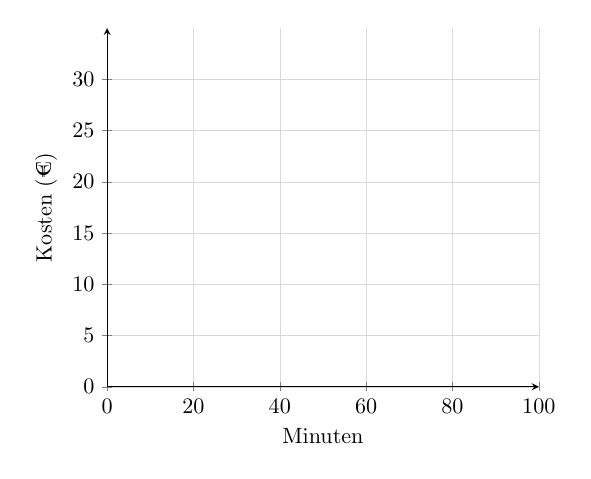
\begin{tikzpicture}[scale=0.8]
                \begin{axis}[
                    axis lines = left,
                    xlabel = {Minuten},
                    ylabel = {Kosten (€)},
                    xmin=0, xmax=100,
                    ymin=0, ymax=35,
                    xtick={0,20,40,60,80,100},
                    ytick={0,5,10,15,20,25,30},
                    grid=major,
                    grid style={line width=0.1pt,draw=gray!30},
                ]
                \end{axis}
            \end{tikzpicture}
        \end{center}

        \item Ab wie vielen Minuten ist Anbieter A günstiger?

        Gleichsetzen: $K_A(x) = K_B(x)$

        \vspace{2.5cm}

        Ab \underline{\hspace{3cm}} Minuten ist Anbieter A günstiger.

    \end{enumerate}

    \item \textbf{Wassertank füllen:}

    Ein Tank fasst 500 Liter. Er wird mit 25 Litern pro Minute gefüllt. Zu Beginn sind bereits 100 Liter im Tank.

    \begin{enumerate}[label=\alph*)]
        \item Funktionsgleichung: $V(t) = $ \underline{\hspace{6cm}} (V in Litern, t in Minuten)

        \item Wie viel Wasser ist nach 8 Minuten im Tank?

        \vspace{1.5cm}

        \item Nach wie vielen Minuten ist der Tank voll?

        \vspace{2cm}

    \end{enumerate}

\end{enumerate}